% !TeX root = RJwrapper.tex
\title{PLreg: An R Package for Modeling Bounded Continuous Data}


\author{by Francisco F. Queiroz and Silvia L.P. Ferrari}

\maketitle

\abstract{%
The power logit class of distributions is useful for modeling continuous data on the unit interval, such as fractions and proportions. It is very flexible and the parameters represent the median, dispersion and skewness of the distribution. Based on the power logit class, Queiroz and Ferrari (2023b, \emph{Statistical Modelling}) proposed the power logit regression models. The dependent variable is assumed to have a distribution in the power logit class, with its median and dispersion linked to regressors through linear predictors with unknown coefficients. We present the R package \textbf{PLreg} which implements a suite of functions for working with power logit class of distributions and the associated regression models. This paper describes and illustrates the methods and algorithms implemented in the package, including tools for parameter estimation, diagnosis of fitted models, and various helper functions for working with power logit distributions, including density, cumulative distribution, quantile, and random number generating functions. Additional examples are presented to show the ability of the \textbf{PLreg} package to fit generalized Johnson SB, log-log, and inflated power logit regression models.
}

\section{Introduction}

Continuous proportion data frequently appear in areas including medicine, biology, and economics. Some concrete examples are vegetation cover fraction, mortality rate, and body fat percentage. Frequently, the interest lies in predicting or explaining the behaviour of proportions from a set of other variables. A natural approach is to use a regression model in which the response variable takes values on the unit interval. The most frequently employed model for bounded data is the beta regression model \citep{FerrariCribariNeto2004} and its extensions. Other models used for bounded continuous data include, for example, rectangular beta \citep{BayesBazanGarcia2012}, simplex \citep{BARNDORFFNIELSEN1991106, ZHANGQIU2014}, log-Lindley \citep{GOMEZDENIZ201449}, CDF-quantile \citep{SmithsonShou2017}, generalized Johnson SB (GJS; \cite{LemonteBazan2016}). Some of these models are implemented in R. For instance, the beta, simplex, and CDF-quantile regression models can be fitted using the packages \CRANpkg{betareg} \citep{Zeileisetal2021}, \CRANpkg{simplexreg} \citep{ZhangQiuShi2016}, and \CRANpkg{cdfquantreg} \citep{Shou2022}, respectively.  The \CRANpkg{gamlss} \citep{Stasinopoulos+Rigby:2007} package can also be used to fit beta and simplex regression models.

Recently, \cite{QueirozFerrari2023} proposed a new class of regression models useful for modeling continuous data with bounded support. The models employ a new class of distributions called power logit (PL), indexed by the median, dispersion and skewness parameters. The PL distributions are constructed from standard symmetric distributions assigned to the power logit transformation of the variable that has support on $(0, 1)$. The power logit transformation is defined in \cite{QueirozFerrari2023} as $t(y; \lambda) = \log[y^\lambda/(1-y^\lambda)]$, for $\lambda>0$ and $y \in (0,1)$; it reduces to the logit transformation when $\lambda=1$. The PL distributions may also depend on an extra parameter that indexes the underlying symmetric distribution; for example, the degrees-of-freedom parameter of the Student-t distribution. The extra parameter adds extra flexibility, which can be used, for example, to deal with outliers. The PL distributions are more flexible than two-parameter distributions, such as the beta, simplex, and CDF-quantile distributions. The class of PL regression models has the GJS regression models as a particular case ($\lambda=1$), with the advantage that the skewness parameter $\lambda$ provides extra flexibility to fit highly skewed data. Applications in real data presented in \cite{QueirozFerrari2023} reveal that the PL regression models are helpful for modeling continuous proportions. 

The new R package \CRANpkg{PLreg} provides a broad set of tools for fitting PL regression models and performing diagnostic analysis. The package is implemented in R and available from the Comprehensive R Archive Network (CRAN) at \url{https:
//CRAN.R-project.org/package=PLreg}. This paper describes and illustrates the methods and algorithms implemented in the package. It also presents some examples to demonstrate the ability of the package to fit generalized Johnson SB, log-log, and inflated power logit regression models.

The remaining of this paper is organized as follows. Section \ref{PLmodel} presents the PL distributions and the associated regression models. Section \ref{sec:implementation} describes the implementation of the PL distributions and the PL regression models in the \CRANpkg{PLreg} package. Section \ref{sec:illustrations} gives detailed illustrations of the use of the \CRANpkg{PLreg} package for modeling continuous bounded data in different scenarios. The paper closes with a brief discussion outlining the features of the \CRANpkg{PLreg} package.

\section{Power logit regression models}\label{PLmodel}

\subsection{Power logit distributions}
The PL distributions \citep{QueirozFerrari2023} are defined from a transformation of a continuous random variable whose distribution is standard symmetric with probability density function $r(z^2)$, $z\in \Reais$, in which $r(z)>0$, for $z \geq 0$, with $\int_0^\infty z^{-1/2} r(z) dz=1$. The function $r(\cdot)$ is called the density generator function. Let $Y$ be a continuous random variable with support $(0,1)$ and let:
%
\begin{equation*}
Z = h(Y; \mu, \sigma, \lambda) = \dfrac{1}{\sigma} \left[ \log \left( \dfrac{Y^\lambda}{1-Y^\lambda} \right) - \log \left( \dfrac{\mu^\lambda}{1-\mu^\lambda} \right)\right],
\end{equation*}
%
where $0< \mu<1$, $\sigma>0$, and $\lambda>0$. If $Z$ has a standard symmetric distribution with density generator function $r(\cdot)$, we say that $Y$ has a PL distribution with parameters $\mu$, $\sigma$ and $\lambda$, and density generator function $r(\cdot)$. We write $Y \sim \mbox{PL} (\mu, \sigma, \lambda; r)$.  The density generator function $r(\cdot)$ may depend on an extra parameter, denoted here by $\zeta$. The distribution of $Y$ depends on the distribution chosen for $Z$. For instance, if $Z$ has a standard normal distribution, then $Y$ has a PL normal distribution; if $Z$ has a standard Student-t distribution with $\zeta$ degrees-of-freedom, then $Y$ has a PL Student-t distribution with extra parameter $\zeta$. 

The probability density function (pdf) of $Y \sim \mbox{PL} (\mu, \sigma, \lambda; r)$ is:
%
\begin{equation*}
f_Y(y; \mu, \sigma, \lambda)= \frac{\lambda}{\sigma y(1-y^\lambda)} r (z^2), \quad y \in (0,1),
\end{equation*}
%
where $z=h(y; \mu, \sigma, \lambda)$. The cumulative distribution function (cdf) of $Y$ is $F_Y(y; \mu, \sigma, \lambda) = R(z)$, where $R(\cdot)$ is the cdf of $Z$.

The GJS class of distributions is a particular case of the PL distributions when $\lambda =1$. Other particular cases are the logit normal distribution \citep{Johnson1949}, the L-Logistic distribution \citep{daPazetal2019}, and the logit slash distribution \citep{Korkmaz2020}, obtained by taking $\lambda =1$ and $Z$ as a standard normal, type II logistic, and slash random variable, respectively.


The PL distributions have some interesting properties. For instance, the parameters $\mu$, $\sigma$ and $\lambda$ represent the median, dispersion and skewness of the distributions, and they have as a limiting case when $\lambda \rightarrow 0^+$, the class of log-log distributions, defined in \cite{QueirozFerrari2023}.


\subsection{Power logit regression models}

The PL regression models are defined as follows. Let $Y_1,\ldots,Y_n$ be $n$ independent random variables, where $Y_i \sim \text{PL}(\mu_i, \sigma_i, \lambda; r)$, for $i=1,\ldots,n$, and
%
\begin{equation}\label{linkfun}
\begin{split}
d_1 (\mu_i) &= \bm{x_i}^{\top} \bm{\beta} = \eta_{1i}, \\ 
d_2 (\sigma_i) &= \bm{s_i}^{\top} \bm{\tau} = \eta_{2i},\\
\end{split} 
\end{equation}
%
where $\bm{\beta}=(\beta_1, \ldots, \beta_p)^{\top} \in \Reais^p$, $\bm{\tau}=(\tau_1, \ldots, \tau_q)^{\top} \in \Reais^q$ and $\lambda>0$ are the unknown parameters, which are assumed to be functionally independent and $p+q+1<n$; $\eta_{1i}$ and $\eta_{2i}$ are the linear predictors; $\bm{x}_i = (x_{i1}, \ldots, x_{ip})^{\top}$ and $\bm{s}_i = (s_{i1}, \ldots, s_{iq})^{\top}$ are the covariates. We assume that $\textbf{X}=[\bm{x}_1,\ldots,\bm{x}_n]^\top$ and $\textbf{S}=[\bm{s}_1,\ldots,\bm{s}_n]^\top$ have column rank $p$ and $q$, respectively. In addition, we assume that the link functions $d_1:(0,1)\to\Reais$ and
$d_2:(0,\infty)\to\Reais$ are strictly monotonic and twice differentiable. Some examples of link functions for the median submodel are: $d_1(\mu) = \log \{\mu/(1-\mu)\}$ (logit); $d_1(\mu) = \Phi^{-1}(\mu)$ (probit), where $\Phi^{-1}(\cdot)$ is the cdf of a standard normal random variable; $d_1(\mu) = - \log \{ - \log \mu \}$ (log-log); and $d_1(\mu) = \log \{ - \log(1-\mu)\}$ (complementary log-log). For the dispersion submodel, the log link, $d_2(\sigma) = \log \sigma$, is the natural choice.

The log-log regression models are a limiting case of the PL regression models when $\lambda \rightarrow 0^+$. The GJS regression models \citep{LemonteBazan2016} are obtained by taking $\lambda = 1$. 

The estimation of $\bm{\theta}=(\bm{\beta}^{\top},\bm{\tau}^{\top}, \lambda)^{\top}$ is based on the maximum likelihood approach. The log-likelihood function of $\bm{\theta}$ for the observed sample $y_1,\ldots,y_n$ is:
%
\begin{equation*}
\ell (\bm{\theta}) = \sum_{i=1}^{n} \ell_i(\mu_i, \sigma_i, \lambda), \label{logver}
\end{equation*}
%
where $\ell_i= \ell_i(\mu_i, \sigma_i, \lambda) = \log \lambda - \log \sigma_i - \log\{1-y_i^\lambda \} + \log\{ r(z_i^2)\} + c$, $z_i = h(y_i; \mu_i, \sigma_i, \lambda)$, and $c$ does not depend on $\bm{\theta}$. The maximum likelihood estimate (mle) of $\bm{\theta}$, denoted by $\widehat{\bm{\theta}}$, can be obtained by solving simultaneously the nonlinear system of equations $\textbf{U}(\bm{\theta}) = \bm{0}_{p+q+1},$ which does not have a closed form, where $\textbf{U}(\bm{\theta})$ is the score function and $\bm{0}_{p+q+1}$ denotes a $(p+q+1)$-dimensional vector of zeros. \cite{QueirozFerrari2023} also proposed a penalized maximum likelihood estimator (pmle), which is recommended when the sample size is small. The pmle, denoted by $\widetilde{\bm{\theta}}$, is computed through numerical optimization as follows.
\begin{itemize}
\item[i.] Compute $\widetilde{\lambda}$ such that:
\[
\widetilde{\lambda} = \underset{\lambda>0}{\mathrm{argmax}}~\ell_p^*(\lambda),
\]
where $\ell_p^* (\lambda)$ is the penalized profile log-likelihood for $\lambda$; see \citet[Equation 7]{QueirozFerrari2023}.
\item[ii.] Compute $\widetilde{\bm{\beta}}$ and $\widetilde{\bm{\tau}}$ by maximizing $\ell(\bm{\beta}, \bm{\tau}, \widetilde{\lambda})$.
\end{itemize}

The extra parameter $\zeta$, if any, is selected by minimizing the overall goodness-of-fit measure $\Upsilon_\zeta$, defined as:
\begin{equation*}
\Upsilon_\zeta = n^{-1} \displaystyle \sum_{i=1}^n | \Phi^{-1}[R(\widetilde{z}^{(i)})] - \upsilon^{(i)}|,
\end{equation*}
where $\widetilde{z}^{(i)}$ is the $i$th order statistic of $\widetilde{z}$, $\upsilon^{(i)}$ is the mean of the $i$th order statistic in a random sample of size $n$ of the standard normal distribution and $\Phi(\cdot)$ is the cdf of the standard normal distribution. Alternatively, $\zeta$ may be selected by maximizing $\ell(\tilde{\bm{\theta}})$.

Some diagnostic tools for the PL regression models are presented in \cite{QueirozFerrari2023}, including quantile, deviance, and standardized residuals, local influence methods, and a generalized leverage measure. Applications and further details on inference methods are found in \cite{QueirozFerrari2023}. 


\section[R code]{R implementation} \label{sec:implementation}

The \CRANpkg{PLreg} package allows fitting the PL regression models. The package is organized in a similar way to other packages for fitting regression models, such as \CRANpkg{betareg} and \CRANpkg{simplexreg}. The estimation process is based on the likelihood theory, and two estimators are available: the mle and the pmle. Diagnostic tools for evaluating the fitted model are also implemented. Currently, the package includes methods for computing three types of residuals: quantile, deviance, and standardized residuals. Local influence measures, leverage measures, and goodness-of-fit statistics are also available. Additionally, the package supports PL regression models with the skewness parameter $\lambda$ fixed, i.e., the package also allows
fitting GJS and log-log regression models. 

\subsection[R code]{Power logit distributions in the \CRANpkg{PLreg} package}

Currently, the \CRANpkg{PLreg} package includes seven distributions of the PL class: the PL normal, PL Student-t, PL power exponential, PL slash, PL hyperbolic, PL sinh-normal, and PL type II logistic distributions. \CRANpkg{PLreg} provides the \fct{dPL}, \fct{pPL}, and \fct{qPL} functions to compute the probability density function, cumulative distribution function and quantile function of the PL distributions. Also, the \fct{rPL} function may be used to generate random samples of variables with a PL distribution. The basic usages of these functions are:
\begin{Scode}
dPL(x, mu, sigma, lambda, zeta = 2, family, log = FALSE)

pPL(q, mu, sigma, lambda, zeta = 2, family, lower.tail = TRUE, log.p = FALSE)

qPL(p, mu, sigma, lambda, zeta = 2, family, lower.tail = TRUE, log.p = FALSE)

rPL(n, mu, sigma, lambda, zeta = 2, family)
\end{Scode}
The main arguments for these functions are \code{mu}, \code{sigma}, \code{lambda} and \code{family}, specifying the parameters $\mu$, $\sigma$, and $\lambda$ and the corresponding density generator function $r(\cdot)$, that is, the distribution of the symmetric distribution $Z$. If \code{lambda = 0}, those functions provide results for the log-log distributions. If the density generator function depends on an extra parameter, its value must be specified in the \code{zeta} argument. On the other hand, if it does not depend on an extra parameter, the argument \code{zeta} is ignored. The arguments \code{x} and \code{q} are the vector of quantiles, \code{p} is a vector of probabilities, and \code{n} is the number of random numbers to be generated. Other arguments are \code{log}, \code{log.p} and \code{lower.tail}. If \code{log = TRUE}, then the logarithm of the probability density function will be returned. If \code{log.p = TRUE}, then the logarithm of the cumulative distribution function will be returned and the quantile function will be computed for $\exp(p)$. If \code{lower.tail = FALSE}, then one minus the cumulative distribution function will be returned and the quantile function will be computed for $1-p$. 

In the following, we present the density generator function of all PL distributions implemented in the \CRANpkg{PLreg} package:
\begin{itemize}
\item PL normal (\code{family = "NO"}): $r(z) = (2\pi)^{-1/2}\exp(-z/2)$;
\item PL Student-t (\code{family = "TF"}): $r(z) = \zeta^{\zeta/2}B(1/2,\zeta/2)^{-1}(\zeta + z)^{-(\zeta+1)/2}$, $\zeta>0$ and $B(\cdot,\cdot)$ is the beta function;
\item PL type II logistic (\code{family = "LO"}): $r(z) = \exp\{ - z^{1/2} \}(1 + \exp\{ - z^{1/2} \})^{-2}$;
\item PL power exponential (\code{family = "PE"}): $r(z) = \zeta/[p(\zeta) 2^{1 + 1/\zeta} \Gamma(1/\zeta)] \times$
\\$ \exp\left\{-z^{\zeta/2}/(2 p(\zeta)^\zeta) \right\}$, $\zeta>0$ and $p(\zeta)^2 = 2^{-2/\zeta} \Gamma(1/\zeta)/\Gamma(3/\zeta)$;
\item PL slash (\code{family = "SLASH"}): $r(z) = (\zeta/\sqrt{2\pi}) \left( z/2 \right)^{-(\zeta + 1/2  )} G\left( \zeta + 1/2, z/2 \right)$, for $z>0$, and $r(z) = 2\zeta/[(2\zeta+1)\sqrt{2\pi}]$, for $z=0$, where $\zeta>0$ and $G(a,x) = \int_0^x t^{a-1}e^{-t}dt$ is the lower incomplete gamma function. When $\zeta = 1$ the slash distribution coincides with the canonical slash distribution;
\item PL hyperbolic (\code{family = "Hyp"}): $r(z) = \exp\left\{ - \zeta \sqrt{1+z} \right\}/(2 \zeta K_1(\zeta))$, with $K_s(\zeta) = \int_0^\infty \frac{x^{s-1}}{2}\times$
\\$ \exp\{ -\frac{\zeta}{2} \left(x + \frac{1}{x} \right) \} \dd x$, is the modified Bessel function of third-order and index $s$.
\item PL sinh-normal (\code{family = "SN"}): $r(z) = 1/(\zeta \sqrt{2 \pi}) \cosh(z^{1/2}) \exp\left[ - 2/\zeta^2 \sinh^2 (z^{1/2}) \right]$, where $\zeta>0$ and $\sinh(\cdot)$ and $\cosh(\cdot)$ represent the hyperbolic sine and cosine functions, respectively.
\end{itemize}

Figure~\ref{fig:Fig1} illustrates the use of the \fct{rPL} and \fct{dPL} functions showing the distribution of random numbers generated from PL hyperbolic distributions with $\zeta=1.2$.


\begin{figure}[t!]
\centering
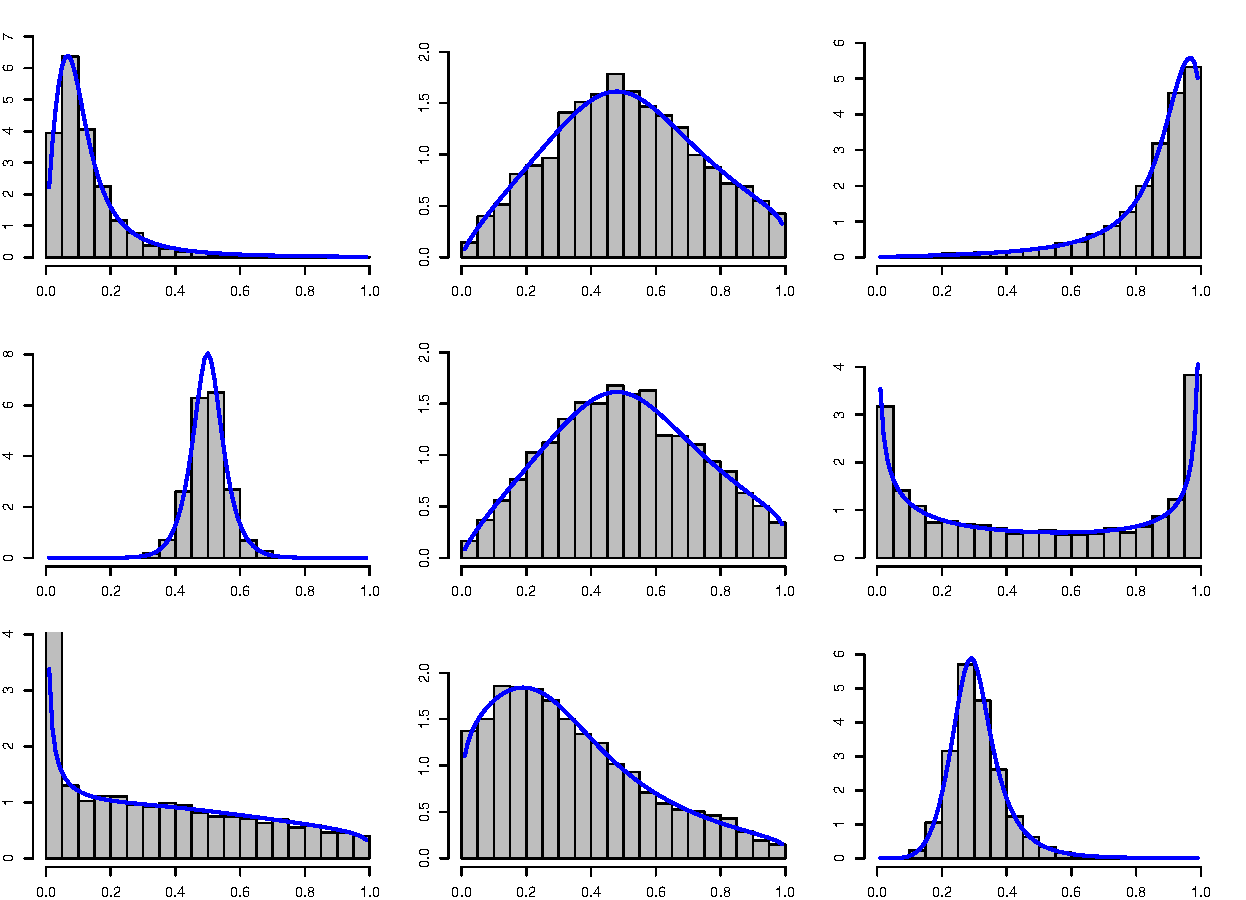
\includegraphics[scale=0.5]{figures/Fig1}
\caption{\label{fig:Fig1} Histograms of random numbers of the PL hyperbolic distributions with $\zeta = 1.2$ with different values for $\mu$, $\sigma$, and $\lambda$. First line: $\mu = (0.1, 0.5, 0.9)$, $\sigma=1$, $\lambda=1.5$; second line: $\mu = 0.5$, $\sigma=(0.2, 1, 3)$, $\lambda=1.5$; third line: $\mu = 0.3$, $\sigma=1$, $\lambda=(0.01, 1, 5)$. Solid lines are
corresponding to the respective PL hyperbolic density.}
\end{figure}

\subsection{Power logit regression models}

The main model-fitting function of the \CRANpkg{PLreg} package is \fct{PLreg}, which is similar to the other functions for implementing regression models in R. The basic usage of the \fct{PLreg} function is:
\begin{Scode}
PLreg(formula, data, subset, na.action, 
 family = c("NO", "LO", "TF", "PE", "SN", "SLASH", "Hyp"), zeta = NULL, 
 link = c("logit", "probit", "cloglog", "cauchit", "log", "loglog"), 
 link.sigma = NULL, type = c("pML", "ML"), control = PLreg.control(...), 
 model = TRUE, y = TRUE, x = FALSE, ...)
\end{Scode}

The argument formula may comprise three parts (separated by the symbols ``\code{~}'' and ``\code{|}''), namely: the observed response variable with values on $(0,1)$, the linear predictor of the median submodel and the linear  predictor of the dispersion submodel (for further details about the \code{formula} argument, see \cite{ZeileisCroissant2010}). For instance,  \code{formula = y ~ x1 + x2 + x3 | z1 + z2}  describes $y$ for the response variable, $x_1$, $x_2$, and $x_3$ for the median submodel, and $z_1$ and $z_2$ for the dispersion submodel. The model is fitted with constant dispersion if the third part of the argument \code{formula} is omitted. So, a PL regression model with constant dispersion may be specified either by \code{formula = y ~ x1 + x2 + x3} or \code{formula = y ~ x1 + x2 + x3 | 1}. The available link functions for the median submodel are \code{"logit"}, \code{"probit"}, \code{"cloglog"}, \code{"cauchit"}, and \code{"loglog"}. For the dispersion submodel, two link functions are allowed: \code{"log"} and \code{"sqrt"}. The default link functions are \code{"logit"} for the median submodel and \code{"log"} for the dispersion submodel. There are two other important arguments: \code{family} and \code{zeta}. The argument \code{family} specifies the symmetric distribution used for generating the PL model; the currentlu supported families are \code{"NO}, \code{"LO"}, \code{"TF"}, \code{"PE"}, \code{"Hyp"}, \code{"SN"}, and \code{"SLASH"}. For the \code{"TF"}, \code{"PE"}, \code{"Hyp"}, \code{"SN"}, and \code{"SLASH"} families the extra parameter must be specified in the \code{zeta} argument.

The estimation process is carried out via \fct{optim} with control options set in \fct{PLreg.control}. It is based on the maximum likelihood method. Currently, two estimators are supported: the usual maximum likelihood estimator (\code{"ML"}) and a penalized maximum likelihood estimator (\code{"pML"}); this should be specified in the \code{type} argument. If the skewness parameter ($\lambda$) is fixed, only the usual maximum likelihood estimator is supported. In this case, a value should be specified in the control argument through the \fct{PLreg.control} function. For instance, \code{control = PLreg.control(lambda = 1)} and \code{control = PLreg.control(lambda = 0)} lead to the GJS and the log-log regression models, respectively; note that $\lambda=0$ represents $\lambda \to 0^+$. Also, if \code{type = "ML"}, \fct{optim} uses analytical gradients in the iterative process; if \code{type = "pML"}, analytical gradients are used only in the iterative process to estimate the parameters of the median and dispersion submodels. By default, the starting values are chosen as described in \cite{QueirozFerrari2023}, but they may be user-supplied through the \fct{PLreg.control} function. 

Once the model has been fitted, an object of \code{S3} class \class{PLreg} is produced. A list of some of the components of this object is presented in Table~\ref{tab:components}. The complete list can be obtained in the reference manual of the package \citep{QueirozFerrari2022}. Several methods are available for objects of class \class{PLreg}. The \fct{summary} method presents a standard output, with coefficient estimates, standard errors, partial Wald statistics and $p$~values for the regression coefficients, as well as the overall goodness-of-fit measure ($\Upsilon_\zeta$), the pseudo $R^2$, and other metrics. The argument \code{type} in \fct{summary} specifies the type of residuals included in the output: \code{"standardized"}, \code{"quantile"} or \code{"deviance"}. The \fct{plot} method draws graphs for diagnostic and influence analyses. Table~\ref{tab:methods} presents a list with all the available functions and methods.

The \fct{extra.parameter} function can be used to select the extra parameter of some PL models. The basic use is as follows:
\begin{Scode}
extra.parameter(object, lower, upper, grid = 10)
\end{Scode}
This function provides a graph of \code{-2loglik} and $\Upsilon_\zeta$ as functions of $\zeta$, the extra parameter. The \code{object} argument is an object of class \class{PLreg}; \code{lower} and \code{upper} are the lower and upper limits of the interval for the extra parameter, respectively; and \code{grid} is the number of values of the extra parameter for which the measures are evaluated.

\begin{table}[t!]
\centering
\begin{tabular}{lp{10.4cm}}
\hline
Component & Description  \\
\hline
\texttt{coefficients}     & {list of the fitted model coefficients.} \\
\texttt{residuals}        & {vector of raw residuals.} \\
\texttt{fitted.values}    & {vector of the fitted values (fitted median for each observation).} \\
\texttt{optim}            & {list with the \fct{optim} output. For unfixed $\lambda$, if \code{type = "pML"}, the output is based on the iterative process for estimating $\bm{\beta}$ and $\bm{\gamma}$; and, if \code{type = "ML"}, it is based on the iterative process for estimating the whole parameter vector.} \\
\texttt{family}           & {character specifying the underlying symmetric distribution.} \\
\texttt{method}           & {optimization method used in \fct{optim}. Default is \code{"BFGS"}.} \\
\texttt{control}          & {control arguments passed to \fct{optim}.} \\
\texttt{start}            & {vector with the starting values used to initialize the optimization process.} \\
\texttt{nobs}             & {number of observations.}   \\
\texttt{df.null}          & {residual degrees of freedom in the null model (constant median and dispersion).}\\
\texttt{df.residual}  & {residual degrees of freedom in the fitted model.}\\
\texttt{lambda}           & {value of the skewness parameter $\lambda$ (\code{NULL} when $\lambda$ is not fixed).}   \\
\texttt{loglik}           & {log-likelihood of the fitted model.}   \\
\texttt{loglikp}           & {penalized profile log-likelihood for $\lambda$.}   \\
\texttt{vcov}             & {covariance matrix of all the parameters.}   \\
\texttt{pseudo.r.squared} & {pseudo R-squared value.}   \\
\texttt{Upsilon.zeta}     & {an overall goodness-of-fit measure.}   \\
\texttt{link}             & {a list with elements \code{"median"} and \code{"dispersion"} containing the link objects for the respective models.}   \\
\texttt{converged}        & {logical value indicating whether the optimization converged successfully.}   \\
\texttt{zeta}             & {a numeric specifying the value of $\zeta$ used in the estimation process. }   \\
\texttt{type}             & {a character specifying the estimation method used.}   \\
\texttt{v}                & {a vector with the $v(z)$ values for all the observations; see \cite{QueirozFerrari2023} for details.}   \\
 \hline
\end{tabular}
\caption{\label{tab:components} List of the components of an object of the \class{PLreg} class.}
\end{table}



\begin{table}[t!]
\centering
\begin{tabular}{lp{10.4cm}}
\hline
Function & Description  \\
\hline
\fct{print}     & prints the coefficients estimates.   \\
\fct{summary}     & output for the fitted model. Returns an object of class \code{"summary.PLreg"} containing the relevant information about the fit and has a \fct{print} method.  \\
\fct{coef}     & extracts the coefficients of the fitted model.\\
\fct{vcov}     & variance and covariance matrix.  \\
\fct{logLik}     & extracts the fitted log-likelihood function.  \\
\fct{model.matrix}     & extracts model matrix of model components.  \\
\fct{AIC}     &  computes information criteria (AIC, BIC, \ldots). \\
\fct{residuals}     & extracts residuals for the fitted model (quantile, standardized and deviance). Default is the standardized residual. \\
\fct{plot}     &  presents some diagnostic plots. Currently, seven types of plots are available: index plot of residuals,  local influence plot based on the case-weight perturbation
scheme, scatter plot of the generalized leverage versus the predicted values, scatter plot of the residuals versus the linear predictors, normal probability plot of the residuals, scatter plot of the predicted values versus the observed
values, and a scatter plot of the $v(z)$ function versus the residuals (for some PL models, $v(z)$ may be interpreted as weights in the estimation process). \\
\fct{influence}     &   provides two influence measures and the generalized leverage for PL regression models. \\
\fct{envelope}     & returns a normal probability plot with simulated envelopes for the residuals.  \\
\fct{extra.parameter}     & provides plots for selecting the extra parameter, if any.  \\
\fct{CI.lambda}     & provides plot of the profile (penalized) likelihood ratio statistics for
$\lambda$. Used to obtain confidence intervals for $\lambda$.  \\
\fct{sandwich}     & provides an estimate for the asymptotic variance and covariance matrix of
the parameter estimators of the PL regression models based on the sandwich estimator.\\
 \hline
\end{tabular}
\caption{\label{tab:methods} List with the methods and functions of an object of the \class{PLreg} class.}
\end{table}

\section[R code]{Examples using the \CRANpkg{PLreg} package} \label{sec:illustrations}

We present some examples to illustrate the features of the \CRANpkg{PLreg} package. We use a simulated dataset and three datasets available in the package: \code{bodyfat\_Aeolus}, \code{Firm}, and \code{PeruVotes}. These analyses were conducted using R version 4.2.2.

\subsection{\code{bodyfat\_Aeolus} data: IID setting}\label{bodyfatiid}

For a simple illustration of the \CRANpkg{PLreg} package, we consider the \code{bodyfat\_Aeolus} data reported in \cite{Chengetal2019}. The dataset used here has 159 observations and was collected in Aeolus Cave, located in East Dorset, Vermont, in the USA. The bats were sampled during the winter of 2009 (covering the winter season from October 2008 to April 2009) and 2016 (October 2015 to April 2016). Here, the interest lies in modeling the proportion of body fat of little brown bats (\code{percentfat}) using the PL distributions. The data can be loaded by:
%
\begin{Schunk}
\begin{Sinput}
R> data("bodyfat_Aeolus", package = "PLreg")
\end{Sinput}
\end{Schunk}
%
and the histogram and boxplot of the response variable are presented in Figure~\ref{fig:Fig2}. Some summary measures of \code{percentfat} are presented below. Note that the distributions of this variable is right-skewed and have some values close to zero, with range $2.5\%-32\%$.
\begin{figure}[t!]
\centering
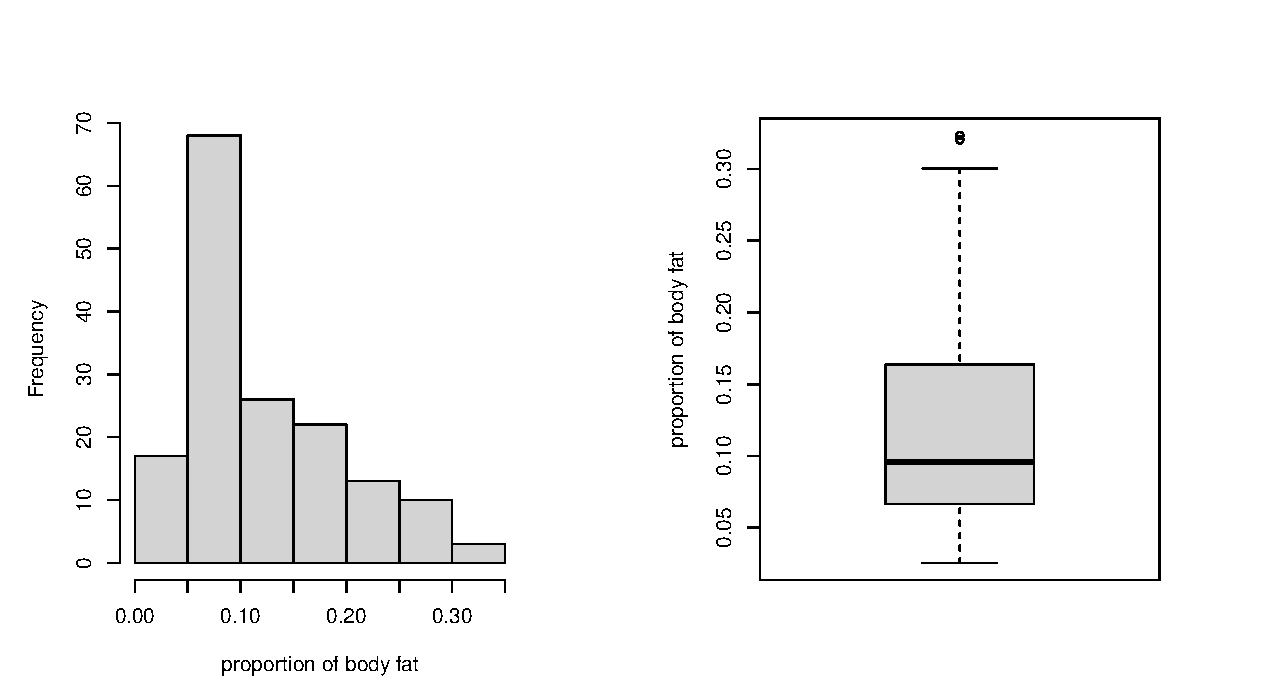
\includegraphics[scale=0.6]{figures/Fig2}
\caption{\label{fig:Fig2} Histogram (left side) and boxplot (right side) of the response variable -- \code{bodyfat$\_$Aeolus} data.}
\end{figure}

\begin{Schunk}
\begin{Sinput}
R> summary(bodyfat_Aeolus$percentfat)
\end{Sinput}
\begin{Soutput}
   Min. 1st Qu.  Median    Mean 3rd Qu.    Max. 
0.02544 0.06658 0.09565 0.12168 0.16371 0.32336
\end{Soutput}
\end{Schunk}

We now fit the \code{percentfat} variable using the PL normal and PL sinh-normal distributions. For the PL sinh-normal distribution, we first fit the distribution with a fixed value of $\zeta$, e.g., $\zeta = 1$, and then we use the \fct{extra.parameter} function to select an optimal value for $\zeta$. In the \CRANpkg{PLreg} package, it can be done via:

\begin{Schunk}
\begin{Sinput}
R> PLNO <- PLreg(percentfat ~ 1, data = bodyfat_Aeolus, family = "NO")
R> PLSN.aux <- PLreg(percentfat ~ 1, data = bodyfat_Aeolus, family = "SN",
+                   zeta = 1)
R> extra.parameter(PLSN.aux, lower = 1, upper = 4, grid = 10)
\end{Sinput}
\begin{Soutput}
Estimates for zeta are: 
zeta.Ups = 1.67
zeta.loglik = 2
\end{Soutput}
\begin{Sinput}
> PLSN <- PLreg(percentfat ~ 1, data = bodyfat_Aeolus, family = "SN",
+               zeta = 1.67)
\end{Sinput}
\end{Schunk}

The \fct{extra.parameter} returns the optimal values for $\zeta$ based on two measures and plots these measures as functions of $\zeta$; see Figure~\ref{fig:Fig3}. We choose \code{zeta = 1.67}. 
\begin{figure}[t!]
\centering
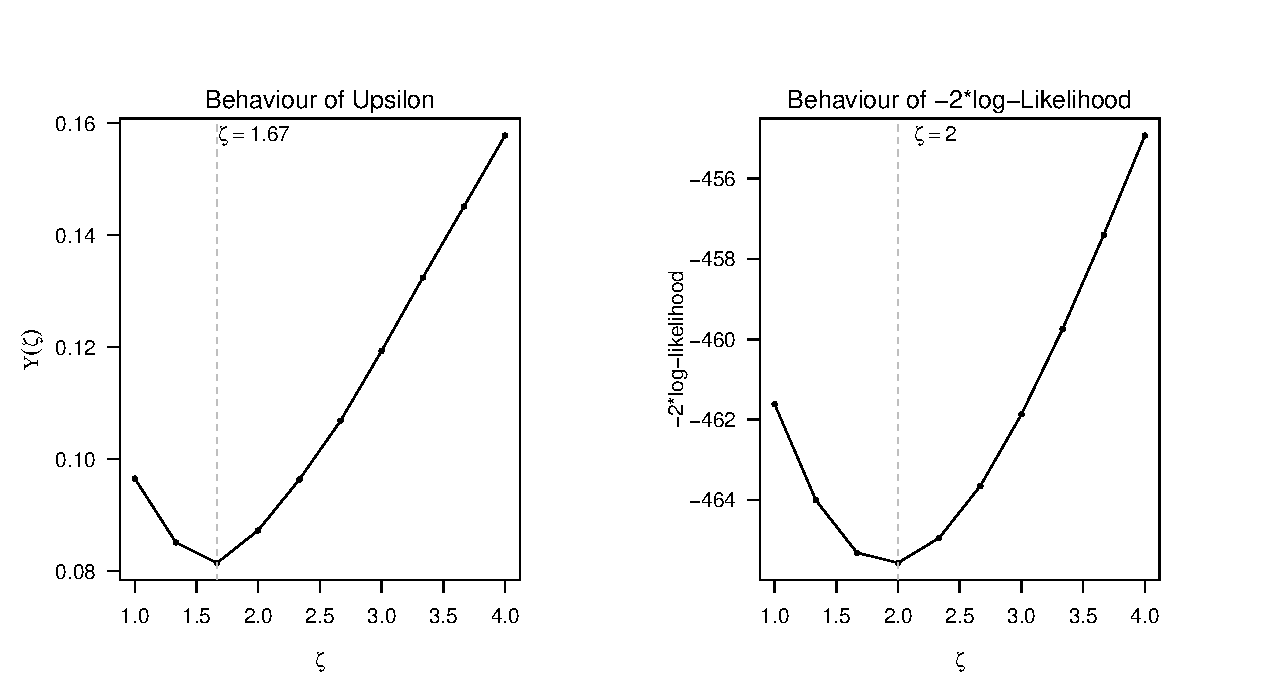
\includegraphics[scale=0.6]{figures/Fig3}
\caption{\label{fig:Fig3} Plot returned by the \fct{extra.parameter} for selecting an optimal value for $\zeta$ of the fit of the PL sinh-normal distribution -- \code{bodyfat\_Aeolus} data.}
\end{figure}

To select between the PL normal and PL sinh-normal distributions, we compute the $\Upsilon_\zeta$ and the AIC for both fits:
\begin{Schunk}
\begin{Sinput}
R> PL_NO <- round(c(PLNO$Upsilon.zeta, AIC(PLNO)), 3)
R> PL_SN <- round(c(PLSN$Upsilon.zeta, AIC(PLSN)), 3)
R> measures <- rbind(PL_NO, PL_SN)
R> colnames(measures) <- c("Upsilon", "AIC")
R> measures
\end{Sinput}
\begin{Soutput}
      Upsilon      AIC
PL_NO   0.114 -443.771
PL_SN   0.082 -453.942
\end{Soutput}
\end{Schunk}

Since the values of $\Upsilon_\zeta$ and AIC for the PL sinh-normal fit are smaller than those of the PL normal fit, we select the PL sinh-normal distribution. The \code{summary} output of the PL sinh-normal fit is presented in the following:
\begin{Schunk}
\begin{Sinput}
R> summary(PLSN)
\end{Sinput}
\begin{Soutput}
Call:
PLreg(formula = percentfat ~ 1, data = bodyfat_Aeolus, family = "SN", 
    zeta = 1.67)

Standardized residuals:
    Min      1Q  Median      3Q     Max 
-2.4654 -0.8318 -0.2065  0.7453  2.0551 

Coefficients (median model with logit link):
            Estimate Std. Error z value Pr(>|z|)    
(Intercept) -2.11477    0.05416  -39.05   <2e-16 ***

Sigma coefficients (dispersion model with log link):
        Estimate Std. Error z value Pr(>|z|)
(sigma)   0.2107     0.4506   0.468     0.64

Lambda coefficient:
         Estimate Std. Error
(lambda)    1.438      0.764
---
Signif. codes:  0 '***' 0.001 '**' 0.01 '*' 0.05 '.' 0.1 ' ' 1 

Family: PL - SN ( 1.67 ) (Power logit sinh-normal)
Estimation method: pML (penalized maximum likelihood)
Log-likelihood:   230 on 3 Df
Upsilon statistic: 0.08151
AIC: -453.9
Number of iterations in BFGS optimization: 9 
\end{Soutput}
\end{Schunk}

The estimated median of the body fat proportion based on the fit is $\exp(-2.11477)/[1+\exp(-2.11477)] \approx 10.8\%$, close to the sample median. Figure~\ref{fig:Fig4} presents the normal probability plot of the quantile residual with simulated envelope for the \code{PLSN} fit and the histogram of \code{percentfat} with the estimated density. These plots can be obtained as follows:
\begin{figure}[t!]
\centering
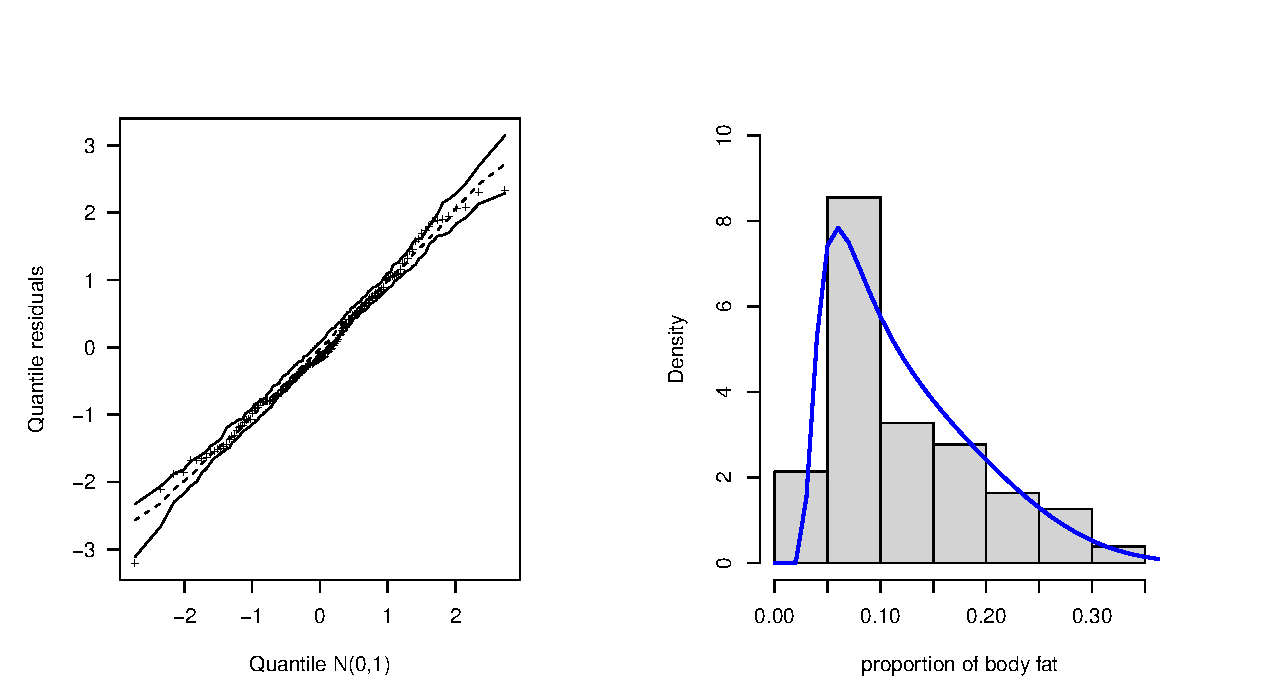
\includegraphics[scale=0.6]{figures/Fig4}
\caption{\label{fig:Fig4} Normal probability plot of the quantile residual with simulated envelope for the \code{PLSN} fit and the histogram of \code{percentfat} with the estimated density -- \code{bodyfat\_Aeolus} data.}
\end{figure}
\begin{Schunk}
\begin{Sinput}
R> set.seed(180123)
R> envelope(PLSN)
R> hist(bodyfat_Aeolus$percentfat, main = " ",
+      xlab = "proportion of body fat", prob = TRUE, ylim = c(0, 10))
R> curve(dPL(x, PLSN$fitted.values[1], exp(PLSN$coefficients$dispersion),
+           PLSN$coefficients$skewness, zeta = 1.67, family = "SN"), 0 , 1, 
+	add = TRUE, lwd = 2, col= "blue")
\end{Sinput}
\end{Schunk}

Using the delta method, an approximated 95\% confidence interval for the median of the body fat proportion is:
\[
\left[\widetilde{\mu} \mp 1.96 \times \mbox{se}(\widetilde{\beta}) \dfrac{\exp(\widetilde{\beta})}{[1+\exp(\widetilde{\beta})]^2}\right] = [ 0.097,~ 0.118].
\]


\subsection[R code]{\code{Firm} data: PL regression model}

We now use the \code{Firm} data to replicate the application presented in \citet[Section 6.2]{QueirozFerrari2023}. The dataset was introduced by \cite{SchmitRoth1990} and presents information on the risk management practices of 73 firms. The response variable is \code{firmcost}, defined as premiums plus uninsured losses as a percentage of the total assets. It is a measure of the firm’s risk management cost-effectiveness. \cite{QueirozFerrari2023} start the analysis with the PL slash regression model with varying dispersion, employing two covariates: \code{sizelog}, the logarithm of total assets,
and \code{indcost}, a measure of the firm’s industry risk. This model can be fitted via: 
\begin{Schunk}
\begin{Sinput}
R> data("Firm", package = "PLreg")

R> Firm_slash2 <- PLreg(firmcost ~ indcost + sizelog | indcost + sizelog,
+			data = Firm, family = "SLASH", zeta = 2)
R> extra.parameter(Firm_slash2, lower = 1, upper = 2.5, grid = 30)
\end{Sinput}
\begin{Soutput}
Estimates for zeta are: 
zeta.Ups = 1.88
zeta.loglik = 1.93
\end{Soutput}
\begin{Sinput}
R> Firm_slash <- PLreg(firmcost ~ indcost + sizelog | indcost + sizelog,
+                    data = Firm, family = "SLASH", zeta = 1.88)
R> summary(Firm_slash)
\end{Sinput}
\begin{Soutput}
Call:
PLreg(formula = firmcost ~ indcost + sizelog | indcost + sizelog, 
	data = Firm, family = "SLASH", zeta = 1.88)

Standardized residuals:
    Min      1Q  Median      3Q     Max 
-2.1220 -0.6253  0.0251  0.6548  4.6194 

Coefficients (median model with logit link):
            Estimate Std. Error z value Pr(>|z|)    
(Intercept)   3.8223     1.0196   3.749 0.000178 ***
indcost       2.3117     0.8062   2.867 0.004140 ** 
sizelog      -0.9082     0.1225  -7.416 1.21e-13 ***

Sigma coefficients (dispersion model with log link):
            Estimate Std. Error z value Pr(>|z|)
(Intercept) -0.56915    0.78874  -0.722    0.471
indcost      0.36623    0.54062   0.677    0.498
sizelog      0.07455    0.09979   0.747    0.455

Lambda coefficient:
         Estimate Std. Error
(lambda)    2.035      1.196
---
Signif. codes:  0 '***' 0.001 '**' 0.01 '*' 0.05 '.' 0.1 ' ' 1 

Family: PL - SLASH ( 1.88 ) (Power logit slash)
Estimation method: pML (penalized maximum likelihood)
Log-likelihood:   123 on 7 Df
Pseudo R-squared: 0.4177
Upsilon statistic: 0.06723
AIC: -232.1
Number of iterations in BFGS optimization: 10
\end{Soutput}
\end{Schunk}

The standard errors presented in the \fct{summary} output is computed from the observed information matrix. \cite{QueirozFerrari2023} employ the sandwich matrix to obtain standard errors. Standard errors are computed from the sandwich matrix by using the \fct{sandwich} function in the \CRANpkg{PLreg} package as follows:
\begin{Schunk}
\begin{Sinput}
R> sand.matrix <- sandwich(Firm_slash)
R> se <- sqrt(diag(sand.matrix)) 
R> se
\end{Sinput}
\begin{Soutput}
        (Intercept)             indcost             sizelog (sigma)_(Intercept) 
         1.30397074          1.05026082          0.16419123          0.54569178 
    (sigma)_indcost     (sigma)_sizelog            (lambda) 
         0.59534023          0.08767362          0.91164845 
\end{Soutput}
\end{Schunk}

All the covariates are statistically significant for the median submodel but not for the dispersion submodel. Then, the authors fit the PL slash regression model with constant dispersion and select $\zeta=2.29$. The model can be fitted as follows: 
\begin{Schunk}
\begin{Sinput}
R> Firm_slash.CD <- PLreg(firmcost ~ indcost + sizelog,
+			data = Firm, family = "SLASH", zeta = 2.29)
R> summary(Firm_slash.CD)
\end{Sinput}
\begin{Soutput}
Call:
PLreg(formula = firmcost ~ indcost + sizelog, 
	data = Firm, family = "SLASH", zeta = 2.29)

Standardized residuals:
    Min      1Q  Median      3Q     Max 
-2.1133 -0.6590  0.0546  0.7168  5.9131 

Coefficients (median model with logit link):
            Estimate Std. Error z value Pr(>|z|)    
(Intercept)   3.8668     0.9994   3.869 0.000109 ***
indcost       2.1330     0.5836   3.655 0.000257 ***
sizelog      -0.9053     0.1120  -8.082 6.38e-16 ***

Sigma coefficients (dispersion model with log link):
        Estimate Std. Error z value Pr(>|z|)
(sigma)   0.1333     0.5331    0.25    0.803

Lambda coefficient:
         Estimate Std. Error
(lambda)    1.788       1.01
---
Signif. codes:  0 '***' 0.001 '**' 0.01 '*' 0.05 '.' 0.1 ' ' 1 

Family: PL - SLASH ( 2.29 ) (Power logit slash)
Estimation method: pML (penalized maximum likelihood)
Log-likelihood:   122 on 5 Df
Pseudo R-squared: 0.4162
Upsilon statistic: 0.06448
AIC:  -234
Number of iterations in BFGS optimization: 15
\end{Soutput}
\end{Schunk}

Normal probability plots of the residuals with simulated envelopes as well as influence plots may be obtained via \fct{envelope} and \fct{influence} functions, respectively. For instance, the plots presented in Figure~\ref{fig:Fig5} are obtained as follows:
\begin{Schunk}
\begin{Sinput}
R> envelope(Firm_slash.CD, type = "quantile")
R> envelope(Firm_slash.CD, type = "deviance")
R> envelope(Firm_slash.CD, type = "standardized")
R> influence(Firm_slash.CD)
\end{Sinput}
\end{Schunk}

\begin{figure}[t!]
\centering
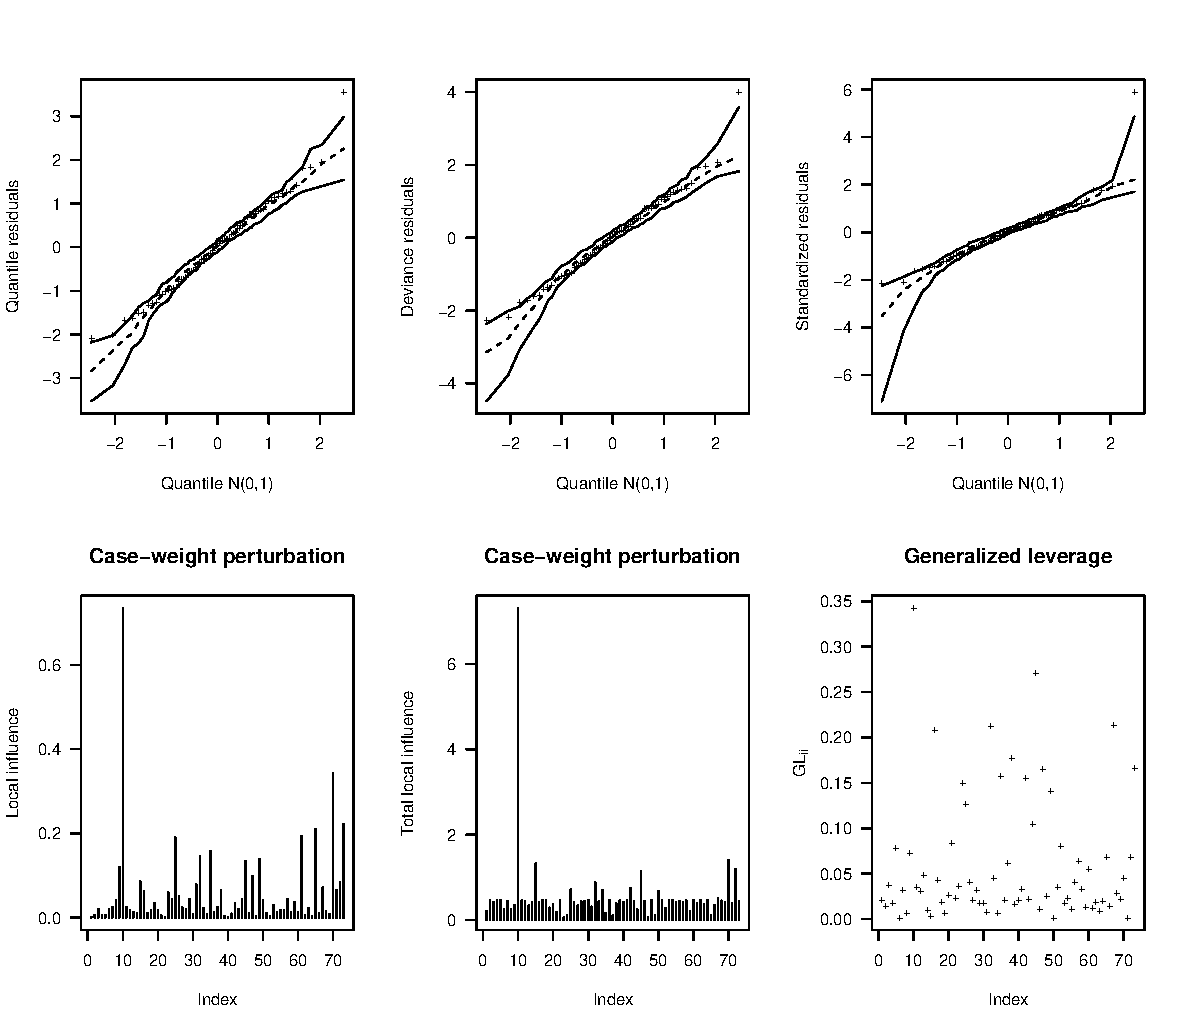
\includegraphics[scale=0.7]{figures/Fig5.pdf}
\caption{\label{fig:Fig5} Normal probability plot of the quantile, deviance and standardized residuals with simulated envelope and influence plots for the \code{Firm\_slash.CD} fit -- \code{Firm} data.}
\end{figure}

Note that one observation is highlighted in almost all the graphics in Figure~\ref{fig:Fig5}. It is the case \#15 and corresponds to a firm with
the highest \code{firmcost} value. \cite{QueirozFerrari2023} conclude that this observation does not significantly influence the fitted model. In fact, the weight of this observation in the estimation process is close to zero --- it may be verified by plotting the weights against the residuals. This plot is presented in Figure~\ref{fig:Fig6} and is obtained via:
\begin{Schunk}
\begin{Sinput}
R> plot(Firm_slash.CD, which = 7)
\end{Sinput}
\end{Schunk}

\begin{figure}[t]
\centering
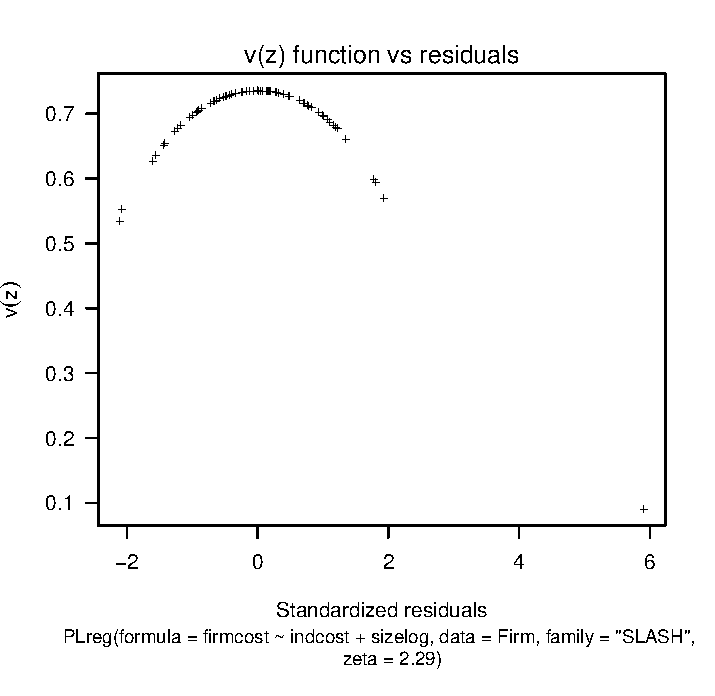
\includegraphics[scale=0.65]{figures/Fig6.pdf}
\caption{\label{fig:Fig6} Plot of the $v(z)$ function against the standardized residual for the \code{Firm\_slash.CD} fit -- \code{Firm} data.}
\end{figure}

The \CRANpkg{PLreg} package allows different link functions for the median submodel. In order to illustrate it, we fit the model with the \code{probit} and \code{cloglog} link functions; for simplicity, we set \code{zeta = 2.29}. We compare the fits through the values of the pseudo $R^2$ and the $\Upsilon_\zeta$ measure as follows:
%
\begin{Schunk}
\begin{Sinput}
R> measures <- sapply(c("logit", "probit", "cloglog"),
+                     function(x){
+                       fit <- update(Firm_slash.CD, link = x)
+                       round(c(fit$pseudo.r.squared, fit$Upsilon.zeta),3)
+                     })
R> rownames(measures) <- c("pseudo R-squared", "Upsilon_zeta")
R> measures
\end{Sinput}
\begin{Soutput}
                 logit probit cloglog
pseudo R-squared 0.416  0.379   0.482
Upsilon_zeta     0.064  0.071   0.069
\end{Soutput}
\end{Schunk}

No model simultaneously has the highest pseudo $R^2$ and the smallest $\Upsilon_\zeta$. Note that the values for the fit with the \code{logit} and \code{cloglog} link functions are close. The \code{probit} link function leads to the smallest pseudo $R^2$ and the highest $\Upsilon_\zeta$; hence it is not recommended.

\subsection[R code]{\code{PeruVotes} data: GJS regression models}

\cite{LemonteBazan2016} use the GJS Student-t regression model to model the proportion of blank votes (\code{votes}) in the 2006 Peruvian general election of an electoral district as a function of the Human Development Index (\code{HDI}). The \code{PeruVotes} dataset contains information on $194$ electoral districts. Recall that the PL regression models with $\lambda=1$ reduce to the GJS regression models. The extra parameter $\zeta$ of the GJS Student-t regression model may be selected using the \fct{extra.parameter} function as in the previous examples. However, to replicate the analysis in \cite{LemonteBazan2016} we fit the PL Student-t regression model with $\zeta=4$ (and $\lambda=1$). Using the  \code{control} argument in the \fct{PLreg} function, we set \code{lambda = 1}: 
%
\begin{Schunk}
\begin{Sinput}
R> data("PeruVotes", package = "PLreg")
R> PV_GJSt <- PLreg(votes ~ HDI | HDI, data = PeruVotes, family = "TF",
+                   zeta = 4, control = PLreg.control(lambda = 1))
R> summary(PV_GJSt)
\end{Sinput}
\begin{Soutput}
Call:
PLreg(formula = votes ~ HDI | HDI, data = PeruVotes, family = "TF", 
    zeta = 4, control = PLreg.control(lambda = 1))

Standardized residuals:
    Min      1Q  Median      3Q     Max 
-5.1247 -0.5838  0.0024  0.5821  4.1666 

Coefficients (median model with logit link):
            Estimate Std. Error z value Pr(>|z|)    
(Intercept)   2.3054     0.2086   11.05   <2e-16 ***
HDI          -6.8075     0.3780  -18.01   <2e-16 ***

Sigma coefficients (dispersion model with log link):
            Estimate Std. Error z value Pr(>|z|)    
(Intercept)  -2.7560     0.7008  -3.933  8.4e-05 ***
HDI           2.1667     1.2422   1.744   0.0811 .  

Fixed skewness parameter (lambda = 1).
---
Signif. codes:  0 '***' 0.001 '**' 0.01 '*' 0.05 '.' 0.1 ' ' 1 

Family: PL - TF ( 4 ) (Power logit Student-t)
Estimation method: ML (maximum likelihood)
Log-likelihood: 352.8 on 4 Df
Pseudo R-squared: 0.5822
Upsilon statistic: 0.06836
AIC: -697.5
Number of iterations in BFGS optimization: 9 
\end{Soutput}
\end{Schunk}
%

As mentioned before, for fixed $\lambda$, the estimation is based on the usual maximum likelihood estimator. The output of the \fct{summary} function may be used to replicate part of Table 2 of \cite{LemonteBazan2016}. The GJS distribution in their paper has a median-precision parameterization, while we use a median-dispersion parameterization. As we are using the logarithmic link function for the dispersion parameter, the estimates for the precision submodel are the negative of those obtained here for the dispersion submodel. 

As the GJS regression models are a particular case of the PL regression models when $\lambda = 1$, an inherent question is whether the dataset supports the assumption that $\lambda =1$. A confidence interval for $\lambda$ may be constructed using the profile penalized likelihood ratio statistic defined by $W_p^*(\lambda) = 2 \{ \ell_p^*(\widetilde{\lambda}) - \ell_p^*(\lambda) \}$, that is asymptotically distributed as $\chi_{1}^2$ \citep{QueirozFerrari2023}. The \fct{CI.lambda} function in the \CRANpkg{PLreg} package provides a plot of $W_p^*(\lambda)$ against $\lambda$ and shows the observed confidence interval for $\lambda$. As an illustration, we fit the PL Student-t regression model with $\zeta=4$ and use the \fct{CI.lambda} function to obtain a 90\% confidence interval for $\lambda$:

\begin{Schunk}
\begin{Sinput}
R> PV_PLt <- PLreg(votes ~ HDI | HDI, data = PeruVotes, family = "TF",
+                  zeta = 4)
R> coefficients(PV_PLt, conf.coef = 0.9)
\end{Sinput}
\begin{Soutput}
        (Intercept)                 HDI (sigma)_(Intercept) 
          2.3050765          -6.8065881          -2.7445500 
        (sigma)_HDI            (lambda) 
          2.0459250           0.9102018 
\end{Soutput}
\begin{Sinput}
R> CI.lambda(PV_PLt)
\end{Sinput}
\begin{Soutput}
The confidence interval for lambda is: (0, 5.4).
\end{Soutput}
\end{Schunk}

The \fct{CI.lambda} function provides the plot presented in Figure \ref{fig:Fig6-1}; the horizontal dashed line indicates the 90\% confidence interval for $\lambda$. Note that the estimated $\lambda$ is close to one, and the confidence interval contains $\lambda=1$. A diagnostic analysis not shown here indicates that the GJS Student-t regression model with $\zeta = 4$ suitably fits the data.

\begin{figure}[t]
\centering
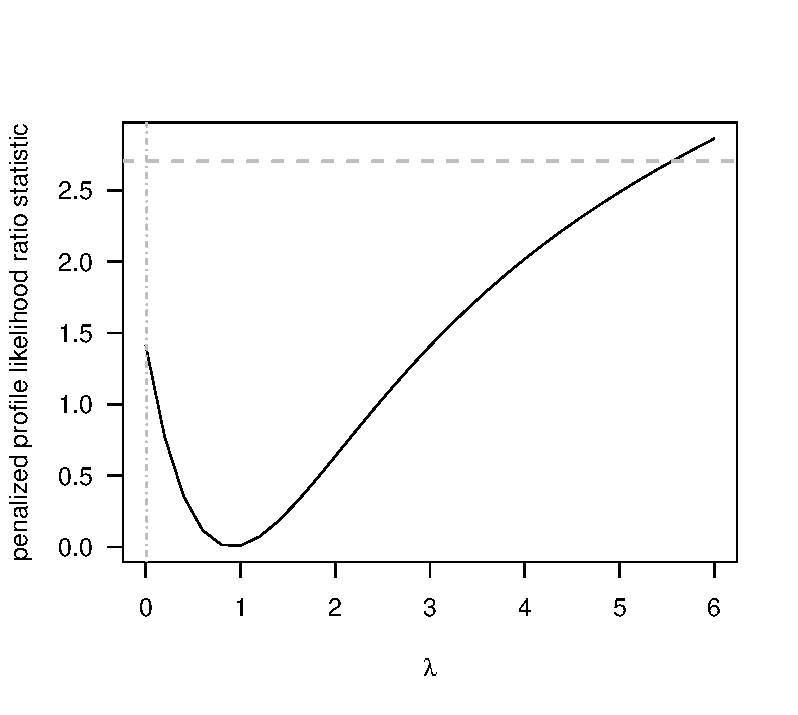
\includegraphics[scale=0.6]{figures/Fig6-1.pdf}
\caption{\label{fig:Fig6-1} Plot of the profile penalized likelihood ratio statistics for $\lambda$ based on the \code{PV\_PLt} fit -- \code{PeruVotes} data.}
\end{figure}

\subsection[R code]{\code{bodyfat\_Aeolus} data: log-log regression models}


We now turn to the \code{bodyfat\_Aeolus} data, introduced in Section~\ref{bodyfatiid}. The interest lies in modelling the proportion of body fat of little brown bats (\code{percentfat}) as a function of the year
(\code{year}, 1 for 2016 and 0 for 2009), sex of the sampled bat (\code{sex}, 1 for male and 0 for female) and the hibernation time (\code{days}), defined as the number of days since the fall equinox. First, we fit the PL normal regression model and print the estimated skewness parameter:
%
\begin{Schunk}
\begin{Sinput}
R> bodyf_PL <- PLreg(percentfat ~ days + sex + year | days + sex + year,
+                    data = bodyfat_Aeolus, family = "NO")
R> bodyf_PL$coefficients$skewness
\end{Sinput}
\begin{Soutput}
    (lambda) 
0.0007122085 
\end{Soutput}
\end{Schunk}

Note that the estimate of $\lambda$ is close to zero. It may indicate the limiting model when $\lambda \to 0^+$ may be reasonable. The log-log normal regression model may be fitted by setting \code{lambda = 0} in the \code{control} argument of the \fct{PLreg} function as follows:
%
\begin{Schunk}
\begin{Sinput}
R> bodyf_loglog <- PLreg(percentfat ~ days + sex + year | days + sex + year,
+                        data = bodyfat_Aeolus, family = "NO",
+                        control = PLreg.control(lambda = 0))
R> summary(bodyf_loglog)
\end{Sinput}
\begin{Soutput}
Call:
PLreg(formula = percentfat ~ days + sex + year | days + sex + 
    year, data = bodyfat_Aeolus, family = "NO", 
    control = PLreg.control(lambda = 0))

Standardized residuals:
    Min      1Q  Median      3Q     Max 
-2.7679 -0.6402  0.0664  0.6834  2.3130 

Coefficients (median model with logit link):
              Estimate Std. Error z value Pr(>|z|)    
(Intercept) -1.1532851  0.0665887 -17.320   <2e-16 ***
days        -0.0094255  0.0005409 -17.427   <2e-16 ***
sexM        -0.0324633  0.0531725  -0.611    0.542    
year2016     0.5039790  0.0581870   8.661   <2e-16 ***

Sigma coefficients (dispersion model with log link):
              Estimate Std. Error z value Pr(>|z|)    
(Intercept) -1.9668123  0.1663712 -11.822   <2e-16 ***
days         0.0007478  0.0012223   0.612   0.5407    
sexM        -0.2873759  0.1145487  -2.509   0.0121 *  
year2016     0.1088719  0.1314918   0.828   0.4077    

Fixed skewness parameter (limiting case lambda -> 0).
---
Signif. codes:  0 '***' 0.001 '**' 0.01 '*' 0.05 '.' 0.1 ' ' 1 

Family: log-log - NO (log-log normal)
Estimation method: ML (maximum likelihood)
Log-likelihood: 323.4 on 8 Df
Pseudo R-squared: 0.6755
Upsilon statistic: 0.05339
AIC: -630.8
Number of iterations in BFGS optimization: 28 
\end{Soutput}
\end{Schunk}
%

Since the log-log normal regression model is more parsimonious than the PL normal regression model, it should be used. One can also consider other models in the log-log class specifying a different family in the \code{family} argument.

\subsection{Simulated data: Inflated PL regression models}

The \CRANpkg{PLreg} package requires that the response variable values are all in the open interval $(0,1)$. It does not allow values at the boundaries, i.e., equal to zero or one. The zero-or-one inflated PL regression models may be employed when the response variable contains values at one of the boundaries. These models may be fitted using the \CRANpkg{PLreg} package in conjunction with the \fct{glm} function.

We say that $Y$ has an inflated PL distribution with parameters $\alpha \in (0,1)$, $\mu \in (0,1)$, $\sigma>0$, and $\lambda>0$ if $\Prob(Y=c) = \alpha$, with $c=0$ or $c=1$, and, with probability $1-\alpha$, $Y \sim \mbox{PL}(\mu, \sigma, \lambda; r)$. In other words, an inflated PL distribution is a mixture of a PL distribution and a degenerate variable in a known value $c$ ($c=0$ or $c=1$). If $c=0$, we have the zero-inflated PL distribution and if $c=1$, the one-inflated PL distribution. The parameters $\mu$, $\sigma$, and $\lambda$ represent the median, dispersion and skewness of the conditional distribution of $Y$ given that $Y \in (0,1)$ and $\alpha$ is the mixture parameter. When $\lambda=1$ the inflated PL distributions reduce to the inflated GJS distributions \citep{QueirozLemonte2021}. If $\lambda \to 0^+$, we have the inflated log-log distributions as a limiting case. 

In the inflated PL regression models, $\mu$ and $\sigma$ are linked to the covariates through linear predictors with unknown coefficients as in Equation~\ref{linkfun}. Likewise, the mixture parameter submodel is $d_0(\alpha_i) = \bm{z}_i^\top \bm{\kappa} = \eta_{0i}$.

One may use the maximum likelihood approach to estimate the parameters of the model, denoted here by $\bm{\theta} = (\bm{\kappa}^\top, \bm{\beta}^\top, \bm{\tau}^\top, \lambda)^\top$. The likelihood function of $\bm{\theta}$ factorizes in two terms, one that depends only on $\bm{\kappa}$ (discrete part) and the other that depends on the remaining parameters (continuous part). Thus, the inference of the discrete part and the continuous part is performed separately. 

We present a brief example with simulated data. We generate 300 observations from the zero-inflated PL normal regression model with a constant dispersion and logit link for the median and mixture parameter submodels:  
%
\begin{Schunk}
\begin{Sinput}
R> n <- 300
R> kappa <- c(-2, 0.5)
R> beta <- c(-1.0, -2.0)
R> sigma <- 0.5
R> lambda <- 2
R> set.seed(25012023)
R> x1 <- runif(n)
R> Z <- X <- matrix(c(rep(1,n), x1), ncol = 2, byrow = FALSE)
R> alpha <- exp(Z%*%kappa)/(1 + exp(Z%*%kappa))
R> mu <- exp(X%*%beta)/(1 + exp(X%*%beta))
R> prob <- runif(n)
R> y <- ifelse((prob <= alpha), 0, rPL(n, mu, sigma, lambda, family = "NO"))
\end{Sinput}
\end{Schunk}
%
The histogram and boxplot of the response variable $y$ are presented in Figure~\ref{fig:Fig7}. We consider fitting the zero-inflated PL normal regression model in which the parameters $\alpha$ and $\mu$ are modeled as a function of \code{x1} through the logit link. To estimate the parameters associated with the discrete part, we fit a binomial regression model in which the response variable is equal to one if $y=0$ and is equal to zero otherwise. The success probability for the $i$-th observation is $\alpha_i$. This model is fitted using the \fct{glm} function \citep{Chambers+Hastie:1992} of the \CRANpkg{stats} package. The continuous part is modeled using the \CRANpkg{PLreg} package. The following code shows how the model is fitted:
\begin{figure}[t!]
\centering
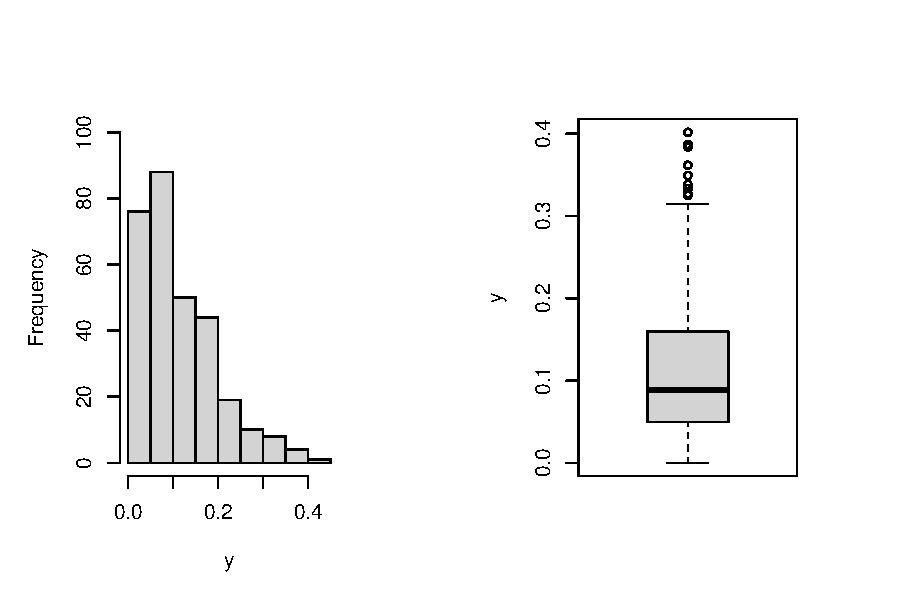
\includegraphics[scale=0.8]{figures/Fig7}
\caption{\label{fig:Fig7} Histogram (left side) and boxplot (right side) of the response variable $y$ -- simulated data.}
\end{figure}


\begin{Schunk}
\begin{Sinput}
R> Ind <- ifelse(y == 0, 1, 0)
R> fit.glm <- glm(Ind ~ x1, family = binomial())
R> fit.PL <- PLreg(y[Ind == 0] ~ x1[Ind == 0], family = "NO", type = "ML")
\end{Sinput}
\end{Schunk}
For estimating the parameters of the discrete part, we consider all the observations. In contrast, to estimate the parameters of the continuous part (PL model), we only consider the observations in $(0,1)$. The estimated coefficients are obtained as follows:
\begin{Schunk}
\begin{Sinput}
R> coefficients(fit.glm)
\end{Sinput}
\begin{Soutput}
(Intercept)          x1 
 -2.1812682   0.9445324 
\end{Soutput}
\begin{Sinput}
R> coefficients(fit.PL)
\end{Sinput}
\begin{Soutput}
    (Intercept)    x1[Ind == 0] (sigma)_(sigma)        (lambda) 
     -0.9608803      -2.1254449       0.3261416       5.3304235
\end{Soutput}
\end{Schunk}

Standard errors and further information may be obtained through the \fct{summary} function. As expected, the estimates of the parameters are close to those used to generate the data. Diagnostic plots for the discrete and continuous parts may be obtained separately by using the \fct{plot} method for the \code{fit.glm} and \code{fit.PL} fits. The overall adequacy of the fitted model may be investigated using the randomized quantile residual \citep{DunnSmyth}. For the inflated PL regression models, the randomized quantile residuals are defined as:
\begin{equation*} 
r_i = \left\{
\begin{array}{rcl}
\Phi ^{-1} (u_i), & & y_i = c,\\
\Phi ^{-1}\left(\widetilde{\alpha}_i \mathbb{I}_{[c,\infty)}(y) + (1- \widetilde{\alpha}_i) F_Y(y_i; \widetilde{\mu}_i, \widetilde{\sigma_i}, \widetilde{\lambda})\right) ,& & y_i \in (0,1),
\end{array}
\right.
\end{equation*}
for $i=1, \ldots, n$, where $c = 0$ or $c=1$ depending on the case. Also, $u_i$ is a random draw from the uniform distribution on the interval $(0, \widetilde{\alpha}_i)$ if $c=0$, and $(1-\widetilde{\alpha}_i, 1)$ if $c=1$. As the \CRANpkg{PLreg} package provides the \fct{pPL} function to obtain the cdf of the PL distributions, the randomized quantile residuals can be easily computed. For the data under investigation, the code below provides the computation of the residuals and the plots presented in Figure \ref{fig:Fig8}.
\begin{Schunk}
\begin{Sinput}
R> alpha  <- fit.glm$fitted.values
R> mu     <- fit.PL$link$median$linkinv(X%*%fit.PL$coefficients$median)
R> sigma  <- fit.PL$link$dispersion$linkinv(fit.PL$coefficients$dispersion)
R> lambda <- fit.PL$coefficients$skewness
R> cdf <- alpha*as.numeric(y >= 0) + (1 - alpha)*pPL(y, mu, sigma, lambda, 
+	family = "NO")
R> res <- ifelse(y == 0, qnorm(runif(length(y), 0, alpha)), qnorm(cdf))
R> plot(res, ylab = "Randomized quantile residuals", pch = "+", ylim = c(-4, 4))
R> abline(h = 2.5, col = "gray", lty = 2)
R> abline(h = -2.5, col = "gray", lty = 2)
R> abline(h = 0, col = "gray", lty = 2)
R> qqnorm(res)
R> qqline(res, col = "gray")
\end{Sinput}
\end{Schunk}
\begin{figure}[t!]
\centering
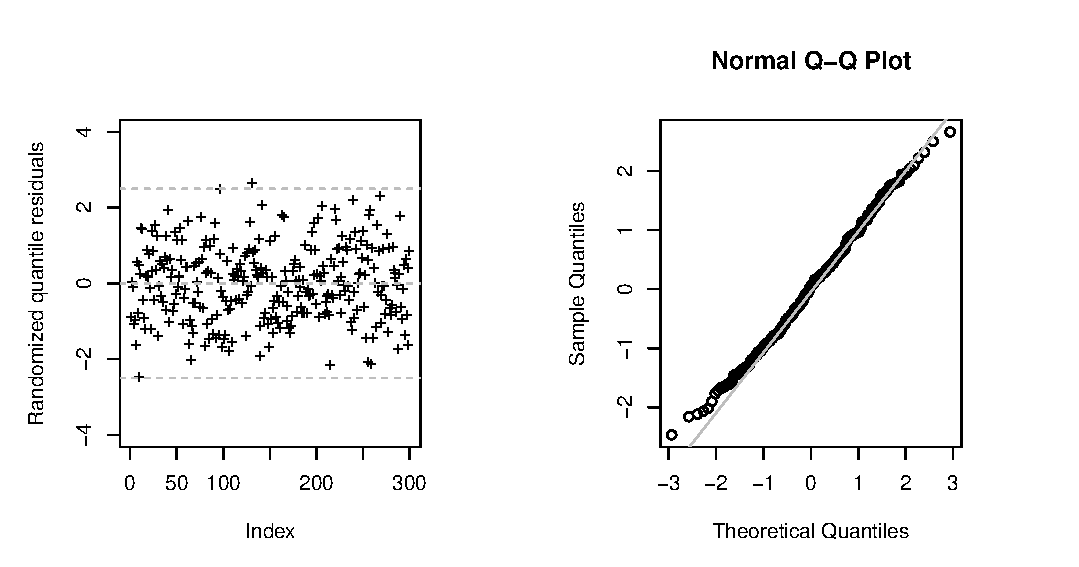
\includegraphics[scale=0.8]{figures/Fig8}
\caption{\label{fig:Fig8} Scatter plot (left side) and quantile-quantile plot (right side) of the randomized quantile residual -- simulated data.}
\end{figure}

We may also fit inflated GJS and inflated log-log regression models specifying \code{lambda = 1} and \code{lambda = 0} in the \code{control} argument of the \fct{PLreg} function, respectively. 


\section{Concluding remarks} \label{sec:summary}

This paper presents the R implementation of the PL regression models available in the \CRANpkg{PLreg} package. The models are suitable for modeling continuous data observed in the open interval (0,1). The package provides tools for likelihood-based inference and diagnostic analysis. Currently, the package includes seven distributions in the PL class, two types of estimators, profile likelihood-based confidence intervals for the skewness parameter, and procedures for selecting the extra parameter, if any. Different residuals and influence methods for performing diagnostic analysis are implemented. The applications in the previous sections illustrate the ability of the package to fit different PL regression models, including the GJS and log-log models.

The response variable for using the \CRANpkg{PLreg} package must lie in the open interval (0,1), as it is an inherent assumption of the PL regression models. A possible approach when the data contain observations in one of the boundaries is to employ the inflated PL regression models, that assume that the response variable has a mixture of a PL distribution and a degenerate distribution at zero or one. A relevant contribution of this paper is to show how the \CRANpkg{PLreg} package can be used to fit and perform diagnostic analysis for inflated PL regression models as well as inflated GJS and log-log regression models.

\section*{Acknowledgments}

We thank the associate editor and the reviewer for their constructive comments on an earlier version
of this article. This study was financed in part by the Coordenação de Aperfeiçoamento de Pessoal de Nível Superior
- Brazil (CAPES) - Finance Code 001 and by the Conselho Nacional de Desenvolvimento Científico e
Tecnológico - Brazil (CNPq). The authors gratefully acknowledge funding provided by CNPq
(Grants No. 150976-2022-4 and No. 305963-2018-0). 



\hypertarget{refs}{}

\bibliography{PLreg.bib}

\address{%
Francisco F. Queiroz\\
Department of Statistics, University of São Paulo\\%
Rua do Matão, 1010\\ 05508-090, São Paulo, Brazil\\ E-mail: email:\href{mailto:felipeq@ime.usp.br}{\nolinkurl{felipeq@ime.usp.br}}\\
%
%
%
%
}

\address{%
Silvia L.P. Ferrari\\
Department of Statistics, University of São Paulo\\%
Rua do Matão, 1010\\ 05508-090, São Paulo, Brazil\\ E-mail: email:\href{mailto:silviaferrari@usp.br}{\nolinkurl{silviaferrari@usp.br}}\\
%
%
%
%
}
